\begin{comment}
  \bibliography{project.bib}
\end{comment}

\chapter{Preliminaries}
\label{cha:preliminaries}

Before we are ready to talk about loading image files, we first need
know how images are represented in a computer.

\section{Color models}
\label{sec:color-models}

\subsection{RGB}
\label{sec:rgb}

There several models for representing color in a computer, but the
most prominent and popular one is by no doubt \textbf{RGB} \index{RGB}

But to understand the RGB color model, we first need to understand
color to begin with. Color is light moving at different
wavelengths. Different colors have different wavelengths. In our eyes
there are cells for perceiving three different wavelengths of light:
Red, Blue and Green(which is what RGB stands for, if you hadn't guessed
it already). There can also be different amounts of red, blue
and green light absorbed by the cells and the colors and also be
mixed, creating new kinds of colors. \cite{neider93:_openg_progr_guide}

\begin{figure}[h]
  \centering
  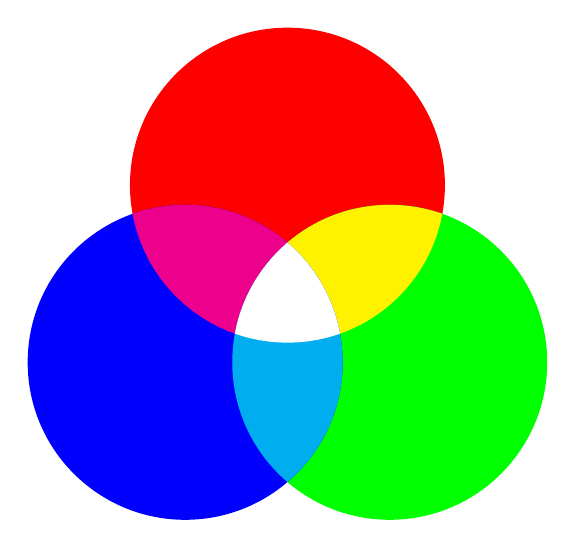
\begin{tikzpicture}

  \draw [draw=none, fill=red] (90:1.5) circle (2cm);
  \draw [draw=none, fill=green] (-30:1.5) circle (2cm);
  \draw [draw=none, fill=blue] (210:1.5) circle (2cm);

  \begin{scope}
    \clip (90:1.5) circle(2cm);
    \draw [draw=none, fill=yellow] (-30:1.5) circle (2cm);
  \end{scope}

  \begin{scope}
    \clip (210:1.5) circle(2cm);
    \draw [draw=none, fill=magenta] (90:1.5) circle (2cm);
  \end{scope}

  \begin{scope}
    \clip (-30:1.5) circle(2cm);
    \draw [draw=none, fill=cyan] (210:1.5) circle (2cm);
  \end{scope}

  \begin{scope} % red + green + blue = white
    \clip (90:1.5) circle(2cm);
    \clip (210:1.5) circle(2cm);
    \draw [draw=none, fill=white] (-30:1.5) circle (2cm);
  \end{scope}
\end{tikzpicture}
  \caption{RGB color model}
  \label{fig:rgb}
\end{figure}

So the RGB color model relies on the fact that all colors are a
mixture of red,blue and green, as it is demonstrated in figure
\ref{fig:rgb}. White is a mixture of red, blue and green, yellow is
mixture of red and green, and so on. The mixing of different amounts
of colors can conveniently enough be specified in numbers very
easily.

\subsection{Alpha channel}
\label{sec:alpha_chan}


But there is actually even more to RGB. There is an extended color
model of RGB that's called RGBA \index{RGBA}(it is sometimes also
called ARGB \index{ARGB}). In this model a new channel is added: the
alpha channel \index{alpha channel}. This new channel represents the
opacity of a color. Opacity is simply the opposite of transparency.  A
low opacity means that the color in question is transparent,
\todo{clarify this part} and that an other color be can be seen
through it.  \cite{porter84_compos_dig_img}.

\section{Color depth}
\label{sec:bit-depth}

\subsection{24-bit color}
\label{sec:24-bit-color}

But how are RGB and RGBA colors represented by a computer? The binary
numeral system is used by computers to store their data. So we can
therefore give every RGB color a value to represent the intensity or
lighttness of a part color. In one popular system every part color of
RGB is given 8-bit of storage. So a full color takes 24-bit is
storage. You can also say that its \textbf{color depth}
\index{color depth} is 24-bits.Observe figure \ref{fig:rgb-bits}. Every color is
here given a 8-bit value. Both the red and the blue channels are given
their highest possible values, 11111111, or in decimal, 255. This
means the channels are given their fullest possible intensities. On
other hand, the green channel has value of 00000000, or simply put,
zero. This means there are no green parts of the colors. The channel
is just dead in this case. If learned anything in color theory, you
should know mixing red and blue gives you yellow. And in the same way,
many, many other possible colors are available. This is just like when
mixed colors in art classes to get different nuances of colors. Only
this time, you can specify the colors mixing \emph{exactly} with
numbers, which is a huge advantage.
\cite{puglia00:_handbook_dig_proj}

\begin{figure}[h]
  \centering
  \newcommand{\bitbox}[3]{
    \filldraw[fill=#2!80!white,draw=black] (#1,0) +(-.2,-.2) rectangle ++(.2,.2);
    \draw (#1,0) node{#3};
  }
  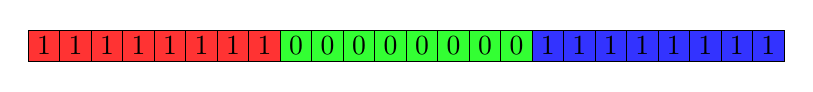
\begin{tikzpicture}
   \foreach \x in {-16.0,-15.6,...,-12.8}
   {
      \bitbox{\x}{red}{1}
   }
   \foreach \x in {-12.8,-12.4,...,-9.6}
   {
      \bitbox{\x}{green}{0}
   }
   \foreach \x in {-9.6,-9.2,...,-6.4}
   {
      \bitbox{\x}{blue}{1}
   }
 \end{tikzpicture}
  \caption{The binary representation of a color}
  \label{fig:rgb-bits}
\end{figure}

% how many different colors?

In RGBA, the alpha channel is stored in the exactly way as the other
three color channel, using a 8-bit number, so there's no need to
further cover this subject.

\subsection{Other colors depths}
\label{sec:other-colors-depths}

\subsection{How many possible colors?}
\label{sec:how-many-possible-colors}

For a color depth of 24-bits there are 256 different combinations for
each color channel, hence there are $256^3 = 16777216$ different
colors for 24-bit color delpth! % combinatorics mention?

% 8-bit color 1-bit color, palettes need to be covered.

\section{Digtal image}
\label{sec:digtal-image}

% raster graphics

% Images can most easily be thought of as an

\printbibliography[heading=subbibliography]